\documentclass[14pt]{extarticle}
\usepackage{amsmath}
\usepackage{amssymb}
\usepackage{tikz}
%\usetikzlibrary{calc}
\usetikzlibrary{trees}
\usepackage{hyperref}
\usepackage{graphicx}
\graphicspath{ {../../chap08/} }
\usepackage[top=0.75in, bottom=0.75in, left=0.75in, right=0.75in]{geometry}
\newcommand*{\Scale}[2][4]{\scalebox{#1}{\ensuremath{#2}}}%
\usepackage[shortlabels]{enumitem}
\usepackage[most]{tcolorbox}
\definecolor{bg}{RGB}{255,249,227}
% \usepackage{showframe}
\title{\vspace{-5ex}Math 208 Section 8.1, 8.2}
\date{\vspace{-10ex}}
\usepackage{multicol}
\setlength{\columnsep}{1cm}


\begin{document}
\maketitle		
\section*{Homework, Reading, and Other}
\begin{itemize}
	\item Section 7.2
	\item Section 7.3, 7.4
	\item Section 8.1, 8.2
\end{itemize}

\section*{Goals}
\begin{itemize}
	\item Understand and derive sample space and events from a statement
	\item Assign simple event probabilities
	\item Calculate compound probabilities
	\item Recognize and calculate union, intersection, and complement probabilities
	\item Relate odds to probabilities and be able to convert.
\end{itemize}

\section*{Probability}
Do you want to win at gambling or any games of chance? Then pay close attention to this chapter. Probability started as a way to understand (and improve odds) in gambling, however, it is now an immensely useful branch of mathematics with applications in practically every field.
\\\\
Probability is critical to understanding risk management, to diversification of investment portfolios, to designing a health care system, to creating plans for retirement, to assessing the risk vs reward for many business decisions, and numerous other applications.

\section*{8.1 Sample Space, Events, and Probability}
In probability theory, an experiment or trial is any procedure that can be infinitely repeated and has a well-defined set of possible outcomes, known as the sample space. An experiment is said to be random if it has more than one possible outcome. For purposes of this section, all experiments are considered random.
\\\\
\textit{Sample Space}, denoted by $S$, is the set all of the possible outcomes of an experiment. An \textit{Event}, denoted by $E$, is the actual outcome of the experiment. An event is always a subset of the sample space.

\subsection{Examples for Sample Space and Events}
Sample Space:
\begin{itemize}
	\item Roll a die: $S=\{1,2,3,4,5,6\}$
	\item Flip a coin twice: $S=\{HH,HT,TH, TT\}$
\end{itemize}
Simple Event:
\begin{itemize}
	\item Roll a 4: $E=\{4\}$
	\item Flip a coin twice and get heads and then tails: $E=\{HT\}$
\end{itemize}
Compound Event:
\begin{itemize}
	\item Roll an even die: $E=\{2,4,6\}$
	\item Flip a coin twice and get more at least 1 heads: $E=\{HH,HT,TH\}$
\end{itemize}
\vspace{5ex}
\textbf{Sample space for rolling two dice}: $S$ is the set of all ordered pairs in the figure.\\
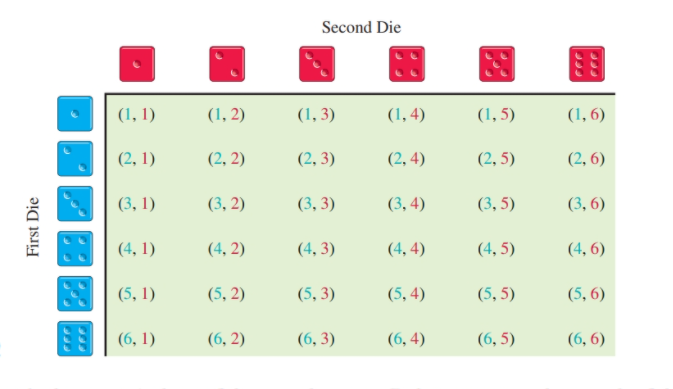
\includegraphics[width=0.9\linewidth]{8-1-5}
\begin{itemize}
	\item What is the event that a sum of 7 is rolled?
	\item $E = \{(6,1), (5,2),(4,3),(3,4),(2,5),(1,6)\}$
	\item What is the event that the sum $<4$?
	\item $E=\{(1,1),(1,2),(2,1)\}$
\end{itemize}

\subsection{Simple Event Probabilities}
\begin{tcolorbox}[enhanced jigsaw,colback=bg,boxrule=0pt,arc=0pt] 
	Given a sample space of $S = \{e_1, e_2, \cdots, e_n\}$ with $n$ simple events. The probability of event $e_i$ is $\mathbf{P(e_i)}$. $P(e_i)$ is subject to two conditions:
	\begin{enumerate}
		\item $P(e_i)$ is between $0$ and $1$, i.e.:
		\begin{align*}
			0 \leq P(e_i) \leq 1
		\end{align*}
		\item The sum of the probabilities of all simple events equals 1, i.e,:
		\begin{align*}
			P(e_1) + P(e_2) + \cdots + P(e_n) = 1
		\end{align*}
	\end{enumerate}
	Any probabilities that satisfy Conditions 1 and 2 are acceptable.
\end{tcolorbox}

\begin{tcolorbox}[enhanced jigsaw,colback=bg,boxrule=0pt,arc=0pt] 
	\textbf{Theorem: Assigning probability under the equally likely assumption} \\\\
	If we assume that each simple event in a sample space S is as likely to occur as any other, then the probability of an arbitrary event E in S is given by
	\begin{align*}
		P(E) = \frac{\text{number of elements in E}}{\text{number of elements in S}} = 
		\frac{n(E)}{n(S)}
	\end{align*}
\end{tcolorbox}


% Set the overall layout of the tree
\tikzstyle{level 1}=[level distance=3.5cm, sibling distance=3.0cm]
\tikzstyle{level 2}=[level distance=3.5cm, sibling distance=1cm]
% Define styles for bags and leafs
\tikzstyle{bag} = [text width=4em, text centered]
\tikzstyle{end} = [circle, minimum width=3pt,fill, inner sep=0pt]
\textbf{Sample space and probabilities for FAIR flipping a coin twice}\\
\begin{tikzpicture}[grow=right, sloped]
	\node[bag] {Start}
	child {
		node[bag] {T}        
		child {
			node[end, label=right:
			{T $\to$ combined event TT $p=\frac{1}{4}$}] {}
		}
		child {
			node[end, label=right:
			{H$\to$ combined event HT $p=\frac{1}{4}$}] {}
		}
	}
	child {
		node[bag] {H}        
		child {
			node[end, label=right:
			{T$\to$ combined event HT $p=\frac{1}{4}$}] {}
		}
		child {
			node[end, label=right:
			{H$\to$ combined event HH $p=\frac{1}{4}$}] {}
		}
	};
\end{tikzpicture}
\begin{itemize}
	\item What is the probability of flipping a head on one flip?
	\item $P(H) = 1/2$
	\item What is the probability of flipping a head or a tail on one flip?
	\item $P(H \text{ or } T) = P(H) + P(T) = 1/2+1/2 = 1$
	\item What is the event two of the same were flipped on two flips? $P(E)$?
	\item $E = \{HH, TT\}$
	\item $P(E) = 1/4 + 1/4 = 1/2$
\end{itemize}

\subsubsection{Assignment from direct experiment}
If a coin were flipped 10,000 times, we would expect heads to turn up about 5,000 times. Likely, the results differed from exactly 5,000 but we would not suspect the coin to be unfair unless there was consistent and substantial difference from 5,000.
\\\\ 
Suppose the results showed 3,750 heads out of 10,000 flips. Now, we suspect that the coin is not fair and may decide to assign probabilities as follows:
\begin{align*}
	&P(H) = \frac{3750}{10000}=0.375 & P(T) = \frac{6250}{10000} =0.625&
\end{align*}
This assignment would be acceptable and reasonable. 

\subsection{Probability of Events}
\begin{tcolorbox}[enhanced jigsaw,colback=bg,boxrule=0pt,arc=0pt] 
	\textbf{Determining the probability of an event, E}
	\begin{itemize}
		\item If $E=\emptyset$, the empty set, then $P(E)=0$.
		\item If E is a simple event, then $P(E)$ is assigned as above.
		\item If E is a compound event, then $P(E)$ is the sum of its simple events.
		\item If $E=S$, the sample space, then $P(E)=1$.
	\end{itemize}
\end{tcolorbox}

\begin{tcolorbox}[enhanced jigsaw,colback=bg,boxrule=0pt,arc=0pt] 
	\textbf{Steps for finding the probability of E}.
	\begin{enumerate}
		\item Determine the sample space, S
		\item Assign probabilities to simple events
		\item Add simple event probabilities to determine compound probability.
	\end{enumerate}
\end{tcolorbox}

\subsubsection{Examples}
\begin{enumerate}
	\item Given two dice, what it the probability of rolling a prime number?
	\begin{itemize}
		\item The sample space, S, is given in the dice chart. $n(S)=36$.
		\item Count the number of primes in the chart. $n(E)=18$ or $n(E)=n(S)/2$.
		\item $P(E) = n(E)/n(S)= 18/36 = 1/2$.
	\end{itemize}
	\item A circular spinner us divided into 15 sectors of equal area, with 6 red, 5 blue, 3 yellow, and 1 green sector. What is the sample space and simple event probabilities?
	\begin{itemize}
		\item The sample space, $S= \{red, blue, yellow, green\}$. With $n(S)=15$.
		\item $P(E =  red) = n(red)/n(S)= 6/15$
		\item $P(E =  blue) = n(blue)/n(S)= 5/15$
		\item $P(E =  yellow) = n(yellow)/n(S)= 3/15$
		\item $P(E =  green) = n(green)/n(S)= 1/15$
		\item Notice that the sum of the probabilities, $\frac{6}{15}+\frac{5}{15}+\frac{3}{15}+\frac{1}{15} = 1$
	\end{itemize}
\end{enumerate}



\section*{8.2 Union, Intersection, and Complement of Event; Odds}
Recall the Venn diagrams and the definitions of Union, Intersection, Disjoint, and Complement from Chapter 7?
\\
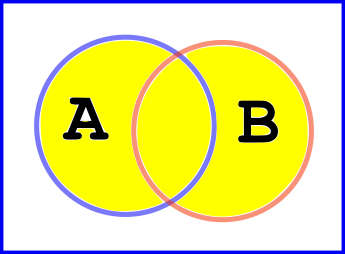
\includegraphics[width=0.3\linewidth]{union}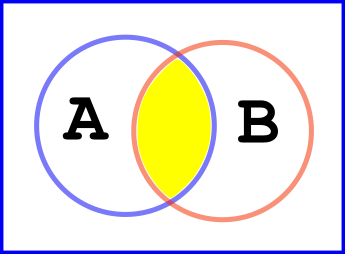
\includegraphics[width=0.3\linewidth]{intersect}
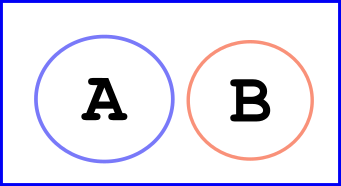
\includegraphics[width=0.3\linewidth]{disjoint}
\\
\subsection{Probabilities}
\begin{tcolorbox}[enhanced jigsaw,colback=bg,boxrule=0pt,arc=0pt] 
	\textbf{Union and Intersection}.
	\begin{enumerate}
		\item \textbf{Event A or B} is $A\cup B = \{e \in S : e \in A \text{ \textbf{or} } e \in B\}$
		\item \textbf{Event A and B} is $A\cap B = \{e \in S : e \in A \text{ \textbf{and} } e \in B\}$
	\end{enumerate}
	\textbf{Probability of the Union}
	$$ P(A\cup B)= P(A) + P(B) -P(A\cap B)$$
	If A and B are disjoint, i.e $A\cap B = \emptyset$, then $P(A\cup B) = P(A) + P(B)$.
\end{tcolorbox}
\begin{tcolorbox}[enhanced jigsaw,colback=bg,boxrule=0pt,arc=0pt] 
	\textbf{Probability of Complement}.
	$$ P(E')= 1-P(E) $$
\end{tcolorbox}

\subsubsection{Examples}
\begin{enumerate}
	\item What is the probability that a number, selected at random from the first 140 positive integers, is divisible by 4 or 6?
	\begin{itemize}
		\item $n(S)= 140$.
		\item Number of integers divisible by 4 is $n(A) = 140/4 =35$
		\item Number of integers divisible by 6 is $n(B) = 140/6 =23$
		\item Number of integers divisible by 4 and 6 is $n(A\cap B) = 140/(6*4) =5$
		\begin{align*}
			P(A\cup B) &= P(A) + P(B) -P(A\cap B) \\
			& = \frac{35}{140}+ \frac{23}{140} - \frac{5}{140} \\
			& = \frac{53}{140}
		\end{align*}
	\end{itemize}
	\item From the previous example, what it the probability that an integer divisible by 4 is not selected?
	\begin{itemize}
		\item $P(E)= 35/140$.
		\begin{align*}
			P(E') &= 1-P(E) \\
			&= 1-35/140 = 105/140 = 3/4
		\end{align*}
	\end{itemize}
	\item (HW 25) With a random selection from 25 balls numbered 1 to 25, what is the probability that the number drawn is odd or a multiple of 4?
	\begin{itemize}
		\item The sample space, $n(S)=25$.
		\item $n(A) = n($multiple of 4$) = 25/4 = 6$.
		\item $P(A)=P($multiple of 4$) =6/25$
		\item $n(B) = n($odd$) = 25/2+1 = 13$.
		\item $P(B)=P($odd$) =13/25$
		\item $A\cap B = \emptyset$.
		\item $P(A\cap B)=0$
		\begin{align*}
			P(A\cup B) &= P(A) + P(B) -P(A\cap B) \\
			& = \frac{6}{25}+ \frac{13}{25} - 0 \\
			& = \frac{19}{25}
			\end{align*}
	\end{itemize}

	\item A shipment of 45 precision parts, including 9 that are defective, is sent to an assembly plant. The quality control division selects 10 at random for testing and rejects the entire shipment if 1 or more in the sample are found to be defective.
	What is the probability that the shipment will be rejected?
	\begin{itemize}
		\item Let E be the event that 1 or more parts in a random sample of 10 are defective.	
		\item Then E´ is the event that no parts in a random sample of 10 are defective.
		\item It is easier to find P(E´) and use that result to find P(E).
		\item $n(S) = _{45}C_{10}$.
		\item $n(E') = _{36}C_{10}$. ($36 = 45-9$)
		\begin{align*}
			P(E) &=1 - P(E') \\
			&= 1 - \frac{_{36}C_{10}}{_{45}C_{10}} \\
			& = 0.92
		\end{align*}
	\end{itemize}

	\item If you are interested, look into the "Birthday Problem"
\end{enumerate}

\subsection{Odds}
When the probability of an event E is known, especially in gaming,we speak of the odds for or against the event instead of the the probability. That is the number of winners to the number of losers. So, the odds of rolling a single die and getting a 2 are: 1 to 5. There is one roll (a 2) in which we win and five rolls (1,3,4,5,6) in which we lose.
\\\\
Odds are used in gaming to make a fair game. In one roll, the odds for rolling a two are 1 to 5. This is a fair bet when: If you bet \$1 on rolling a 2, the house pays \$5 and returns your \$1 bet. You lose your \$1 for any other outcome. 
\\\\
There is a direct relationship between odds and probability.
\begin{tcolorbox}[enhanced jigsaw,colback=bg,boxrule=0pt,arc=0pt] 
	\textbf{Odds $\Leftrightarrow $ Probability}.
	\begin{enumerate}
		\item \textbf{Odds for E} $$= \frac{P(E)}{P(E')}$$
		\item \textbf{Odds against E} $$= \frac{P(E')}{P(E)}$$
		\item \textbf{P(E)} Given the odds are \textit{a to b}, then $$P(E)= \frac{a}{a+b}$$
	\end{enumerate}
\end{tcolorbox}

\subsubsection{Examples}
\begin{enumerate}
	\item Given two dice, what are the odds of rolling 3? What are the odds against rolling 3?
	\begin{itemize}
		\item $P(E) = \frac{n(E)}{n(S)} = \frac{2}{36}$. so that the odds for E are $2:34$ or $1:17$.
		\item The odds against rolling three are $34:2$ or $17:1$
	\end{itemize}
	\item Given the odds against an event are $5:3$, what is $P(E)$?
	\begin{itemize}
		\item The odds for E are $3:5$, then $P(E)=\frac{3}{3+5} = 3/8$
	\end{itemize}
\end{enumerate}



\noindent\rule{\textwidth}{1pt}
{\footnotesize Copyright (C) 2021 Garold Dalton --- Released under GNU General Public License v3.0}


\cleardoublepage


\end{document}
